\section*{ĐỀ TRẮC NGHIỆM CUỐI CHƯƠNG}
\Opensolutionfile{ans}[ans/ans0D6-OT1]
\setcounter{ex}{0}
\subsubsection{Đề số 1}
\begin{ex}%[0D2B1]
	Điểm nào sau đây thuộc đồ thị hàm số $y=x^4+x^3-2x^2+1$?
	\choice
	{\True $M(-2;1)$}
	{$N(1;6)$}
	{$P(-1;1)$}
	{$Q(0;-1)$}
	\loigiai{
		Thay $x=-2$ và $y=1$ vào hàm số $y=x^4+x^3-2x^2+1$, ta thấy thỏa mãn nên điểm $M$ thuộc đồ thị.
	}
\end{ex}

	\begin{ex}%[0D2B1]
		Đồ thị của hàm số $y =f(x) = \heva{
			&2x+1, & \mbox{với } x \le 2 \\&
			- 3, & \mbox{với } x > 2
		}$
		đi qua điểm nào sau đây?
		\choice
		{\True$\left( {0;1} \right)$}
		{$\left( {3;7} \right)$}
		{$\left( {2;-3} \right)$}
		{$\left( {0; - 3} \right)$}
		\loigiai{
		
		}
	\end{ex}
	
	\begin{ex}%[0D2B1]
		Tìm tập xác định của hàm số $y=\dfrac{2x+3}{x^2-x}$.
		\choice{$\mathbb{R}\setminus\{1\}$}
		{$\mathbb{R}$}
		{$\mathbb{R}\setminus\{0\}$}
		{\True $\mathbb{R}\setminus\{0,1\}$}
		\loigiai{
			\begin{itemize}
				\item [$\bullet$] Điều kiện xác định $x^2-x \ne 0 \Leftrightarrow x \ne 0$ và $x \ne 1$.
				\item [$\bullet$] Tập xác định là $\mathbb{R}\setminus\{0,1\}$.
			\end{itemize}
		}
	\end{ex}
	

	
	\begin{ex}%[0D2B1]
		Tìm tập xác định $\mathcal{D}$ của hàm số $y=\dfrac{x-1}{x-2}$.
		\choice
		{\True $\mathcal{D}=\mathbb{R}\setminus\{2\}$}
		{$\mathcal{D}=\mathbb{R}\setminus\{1\}$}
		{$\mathcal{D}=\mathbb{R}$}
		{$\mathcal{D}=\mathbb{R}\setminus\{1;2\}$}
		\loigiai{
				\begin{itemize}
				\item [$\bullet$] Điều kiện xác định $x-2 \ne 0 \Leftrightarrow x \ne 2$.
				\item [$\bullet$] Tập xác định là $\mathbb{R}\setminus\{2\}$.
			\end{itemize}
		}
	\end{ex}
	
	\begin{ex}%[0D2B1]
		Tìm tập xác định $\mathcal{D}$ của hàm số $y=\sqrt{x-2}$.
		\choice
		{$\mathcal{D}=\mathbb{R}\setminus\{2\}$}
		{$\mathcal{D}=(2;+\infty)$}
		{$\mathcal{D}=(-\infty;2)$}
		{\True $\mathcal{D}=[2;+\infty)$}
		\loigiai{
				\begin{itemize}
				\item [$\bullet$] Điều kiện xác định $x-2 \ge 0 \Leftrightarrow x \ge 2$.
				\item [$\bullet$] Tập xác định là $\mathcal{D}=[2;+\infty)$.
			\end{itemize}
		}
	\end{ex}
	
	\begin{ex}%[0D2B1]
		Tìm tập xác định $\mathcal{D}$ của hàm số $y=\dfrac{x-2}{x^2-2x+2}$.
		\choice
		{$\mathcal{D}=\mathbb{R}\setminus\{1\}$}
		{$\mathcal{D}=\mathbb{R}\setminus\{2\}$}
		{\True $\mathcal{D}=\mathbb{R}$}
		{$\mathcal{D}=\mathbb{R}\setminus\{1;2\}$}
		\loigiai{
				\begin{itemize}
				\item [$\bullet$] Điều kiện xác định $x^2-2x+2 \ne 0$ (thỏa với mọi $x \in \mathbb{R}$).
				\item [$\bullet$] Tập xác định là $\mathbb{R}$.
			\end{itemize}
		}
	\end{ex}
	
	

	\begin{ex}%[0D2B1]
		Tìm tập xác định của hàm số $y=\sqrt{3+x}+\sqrt{6-x}$.
		\choice
		{\True $[-3;6]$}
		{$(-3;6)$}
		{$(-\infty;-3)\cup (6;+\infty)$}
		{$\mathbb{R}\backslash(-3;6)$}
		\loigiai{
			\begin{itemize}
				\item [$\bullet$] Điều kiện xác định $\heva{& 3+x \ge 0\\& 6-x \ge 0} \Leftrightarrow -3 \le x \le 6.$
				\item [$\bullet$] Vậy tập xác định là $D=[-3;6]$.
			\end{itemize}
			}
	\end{ex}
	
	\begin{ex}%[0D2K1]
		Tập xác định của hàm số $y=\displaystyle \dfrac{\sqrt{2-2x}}{x^2-1}$ là 
		\choice
		{$\mathscr{D}=(1;+\infty)$}
		{$\mathscr{D}=\mathbb{R} \setminus \{-1;1\}$}
		{\True $\mathscr{D}=(-\infty;1) \setminus\{-1\}$}
		{$\mathscr{D}=(-\infty;1]\setminus \{-1\}$}
		\loigiai{
			\begin{itemize}
				\item [$\bullet$] Điều kiện xác định $\begin{cases}
					2-2x \ge 0 \\ x^2-1 \ne 0
				\end{cases} \Leftrightarrow \begin{cases}
					x \le 1 \\ x \ne \pm 1
				\end{cases} \Leftrightarrow \begin{cases}
					x < 1 \\ x \ne -1.
				\end{cases}$
				\item [$\bullet$] Suy ra tập xác định là $\mathscr{D}=(-\infty;1) \setminus\{-1\}$.
			\end{itemize}
		}
	\end{ex}
	

	\begin{ex}%[0D2B1]
		Tập xác định của hàm số $y=\sqrt{x-1}+\dfrac{2017}{x-3}$ là
		\choice
		{$\mathscr{D}=\left[1;+\infty\right)$}
		{$\mathscr{D}=R\backslash\left\{3\right\}$}
		{\True $\mathscr{D}=\left[1;+\infty\right)\backslash\left\{3\right\}$}
		{$\mathscr{D}=\mathbb{R}$}
		\loigiai{
			\begin{itemize}
				\item [$\bullet$] Hàm số xác định khi
				$\heva{&x-1\ge 0\\&x-3\ne 0}\Leftrightarrow \heva{&x\ge 1\\&x\ne 3}$.
				\item [$\bullet$] Vậy tập xác định là $\mathscr{D}=\left[1;+\infty\right)\backslash\left\{3\right\}$.
			\end{itemize}
			
		}
	\end{ex}
	
	\begin{ex}%[0D2Y2]
		Trong các hàm số sau đây, hàm số nào nghịch biến trên $ \mathbb{R} $?
		\choice
		{\True $y =  - 5x + 3$}
		{$y = 5x + 3$}
		{$y =  - 5 + 3x$}
		{$y = 5x - 3$}
		\loigiai{
			Hàm số $y=ax+b$ nghịch biến trên $\mathbb{R}$ khi $a<0$.
		}
	\end{ex}
	
		\begin{ex}
		Trong các đường biểu diễn sau, đường nào không được coi là đồ thị của một hàm số?
		\boncot
		{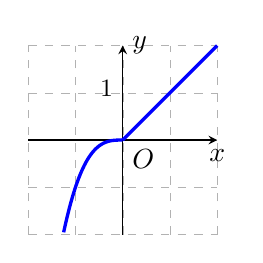
\begin{tikzpicture}[smooth,samples=300,scale=0.6,>=stealth]
				\draw[color=gray!60!white,line width=0.07pt,dashed] (-2,-2) grid (2,2);
				\draw[->] (-2,0)--(2,0) node[below]{$x$};
				\draw[->] (0,-2)--(0,2) node[right]{$y$};
				\draw (0,0) node[below right]{$O$};
				\draw[line width=1.2pt, color=blue,domain=-1.25:0] plot(\x,{(\x)^3});
				\draw[line width=1.2pt,color=blue,domain=0:2] plot(\x,{(\x)});
				\node[left] at (0,1.1) {\small $1$};
		\end{tikzpicture}}
		{ 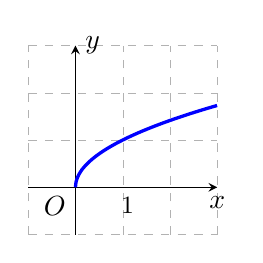
\begin{tikzpicture}[smooth,samples=300,scale=0.6,>=stealth]
				\draw[color=gray!60!white,line width=0.07pt,dashed] (-1,-1) grid (3,3);
				\draw[->] (-1,0)--(3,0) node[below]{$x$};
				\draw[->] (0,-1)--(0,3) node[right]{$y$};
				\draw (0,0) node[below left]{$O$};
				\draw[line width=1.2pt, color=blue,domain=0:3] plot(\x,{(\x)^0.5});
				\node[below] at (1.1,0) {\small $1$};
		\end{tikzpicture}}
		{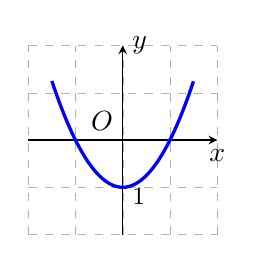
\begin{tikzpicture}[smooth,samples=300,scale=0.6,>=stealth]
				\draw[color=gray!60!white,line width=0.07pt,dashed] (-2,-2) grid (2,2);
				\draw[->] (-2,0)--(2,0) node[below]{$x$};
				\draw[->] (0,-2)--(0,2) node[right]{$y$};
				\draw (0,0) node[above left]{$O$};
				\draw[line width=1.2pt, color=blue,domain=-1.5:1.5] plot(\x,{(\x)^2-1});
				\node[right] at (0,-1.2) {\small $1$};
		\end{tikzpicture}}
		{\True 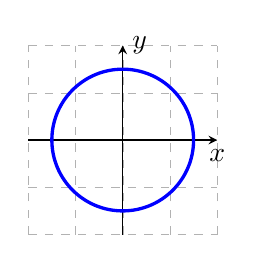
\begin{tikzpicture}[smooth,samples=300,scale=0.6,>=stealth]
				\draw[color=gray!60!white,line width=0.07pt,dashed] (-2,-2) grid (2,2);
				\draw[->] (-2,0)--(2,0) node[below]{$x$};
				\draw[->] (0,-2)--(0,2) node[right]{$y$};
				\draw[line width=1.2pt, color=blue] (0,0) circle (1.5);
		\end{tikzpicture} }
		\loigiai{
			
		}
	\end{ex}
	
	\begin{ex}
		\immini{ Cho hàm số $y=f(x)$ xác định trên $\mathbb{R}$ và có đồ thị như hình bên. Khẳng định nào sau đây đúng?
			\choice
			{Hàm số đồng biến trên khoảng $(0;4)$}
			{\True Hàm số đồng biến trên khoảng $(-1;1)$}
			{ Hàm số đồng biến trên khoảng $(-1;3)$}
			{ Hàm số nghịch biến trên khoảng $(-\infty;0)$}
		}{\hspace{0.5cm}
			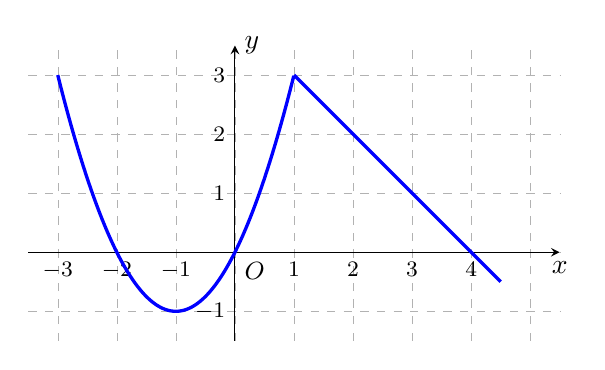
\begin{tikzpicture}[smooth,samples=300,scale=0.75,>=stealth]
				\draw[color=gray!60!white,line width=0.07pt,dashed] (-3.5,-1.5) grid (5.5,3.5);
				\draw[->] (-3.5,0)--(5.5,0) node[below]{$x$};
				\draw[->] (0,-1.5)--(0,3.5) node[right]{$y$};
				\foreach \x in {-3,-2,-1,1,2,3,4}{
					\draw (\x,0) node[below]{\footnotesize $\x$};%Ox
				}
				\foreach \y in {-1,1,2,3}{
					\draw (0,\y) node[left]{\footnotesize $\y$};%Oy
				}
				\draw (0,0) node[below right]{\small $O$};
				\draw[line width=1.2pt, color=blue,domain=-3:1] plot(\x,{(\x+1)^2-1});
				\draw[line width=1.2pt, color=blue,domain=1:4.5] plot(\x,{-(\x)+4});
				%\node[right] at (0.5,-2) {\fbox{$a>0$}};
		\end{tikzpicture}}
		\loigiai{
		}
	\end{ex}


	\begin{ex}%[0D2B3]
		Parabol $y=-x^2+2x$ có đỉnh là
		\choice 
		{\True $I(1;1)$}
		{$I(-1;1)$}
		{$I(-1;2)$}
		{$I(2;0)$}
		\loigiai{
		\begin{itemize}
			\item [$\bullet$] Hoành độ đỉnh $x=-\dfrac{b}{2a}=-\dfrac{2}{2 \cdot (-1)}=1$.
			\item [$\bullet$] Với $x=1$, thay vào hàm số ta tính được $y=1$. Vậy tọa độ đỉnh là $(1;1)$.
		\end{itemize}
		}
	\end{ex}
	
	\begin{ex}%[0D2B3]
		Tìm tọa độ đỉnh $I$ của Parabol $y=x^2-3x+4$.
		\choice{$I(3;3)$}
		{\True $\left(\dfrac{3}{2};\dfrac{7}{4}\right)$}
		{$\left(-\dfrac{3}{2};\dfrac{43}{4}\right)$}
		{$\left(\dfrac{3}{2};-\dfrac{7}{4}\right)$}
		\loigiai{
			\begin{itemize}
				\item [$\bullet$] Hoành độ đỉnh $x=-\dfrac{b}{2a}=\dfrac{3}{2}$.
				\item [$\bullet$] Với $x=\dfrac{3}{2}$, thay vào hàm số ta tính được $y=\dfrac{7}{4}$. Vậy tọa độ đỉnh là $\left(\dfrac{3}{2};\dfrac{7}{4}\right)$.
			\end{itemize}
		}
	\end{ex}
	
	\begin{ex}%[0D2B3]
		\immini{Hình bên là đồ thị của một trong bốn hàm số được cho ở bên dưới. Hàm số đó là hàm số nào?
		\choice
			{$ y =  - {x^2} + 3x - 1 $}
			{$y =  - 2{x^2} + 3x - 1$}
			{\True $y = 2{x^2} - 3x + 1$}
			{$y = {x^2} - 3x + 1$} }{
			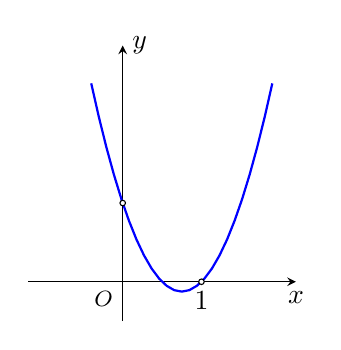
\begin{tikzpicture}[>=stealth] 
			\draw[->] (-1.2,0) -- (2.2,0) node[below] {$x$};
			\draw[->] (0,-0.5) -- (0,3) node[right] {$y$};
			\node at (0,0) [below left] {\footnotesize $O$};
			\draw [domain=-0.4:1.9, blue,thick] plot (\x, {2*((\x)^2)-3*(\x)+1)} );
			\node at (1,0) [below]{$1$};
			\fill[fill=white,draw=black]
			(1,0) circle (1pt) (0,1) circle (1pt);
			\end{tikzpicture}}
		\loigiai{
			\begin{itemize}
				\item [$\bullet$] Từ hình ảnh đồ thị, suy ra $a>0$. Ta loại các phương án có hệ số $a<0$.
				\item [$\bullet$] Mặt khác đồ thị qua điểm $(1;0)$ nên phương án $y = 2{x^2} - 3x + 1$ thỏa mãn.
			\end{itemize}
		}
	\end{ex}
	
	\begin{ex}%[0D2Y3]
		Cho hàm số $y=-2x^2-4x+10$. Tìm khẳng định đúng.
		\choice{Hàm số đồng biến trên khoảng $(-\infty;-2)$ và nghịch biến trên $(-2;+\infty)$}
		{Hàm số nghịch biến trên khoảng $(-\infty;-2)$ và đồng biến trên $(-2;+\infty)$}
		{\True Hàm số đồng biến trên khoảng $(-\infty;-1)$ và nghịch biến trên $(-1;+\infty)$}
		{Hàm số nghịch biến trên khoảng $(-\infty;-1)$ và đồng biến trên $(-1;+\infty)$}
		\loigiai{
			Tọa độ đỉnh $(-1;12)$.\\
			Bảng biến  thiên:
			\begin{center}
				
\begin{tikzpicture}
					\tkzTabInit[nocadre=false, lgt=1, espcl=3]{$x$ /0.7,$y$ /2}{$-\infty$,$-1$,$+\infty$}
					\tkzTabVar{-/ $-\infty$ / ,+/$12$, -/ $-\infty$ /}
				\end{tikzpicture}
			\end{center}
		Từ bảng biến thiên ta được hàm số đồng biến trên khoảng $(-\infty;-1)$ và nghịch biến trên $(-1;+\infty)$.
		}
	\end{ex}
	
	\begin{ex}%[0D2B3]
		\immini{Hàm số nào trong các hàm số sau đây có bảng biến thiên như hình vẽ:
		\choice
		{\True $y = -x^2 + 2x -3$}
		{$y = x^2 +2x -1 $}
		{$y = -x^2 -x -1$}
		{$y = x^2 -x -1$}}{
		
\begin{tikzpicture}
			\tkzTabInit[nocadre=false, lgt=1, espcl=3]{$x$ /0.7,$y$ /2}{$-\infty$,$1$,$+\infty$}
			\tkzTabVar{-/ $-\infty$ / ,+/$-2$, -/ $-\infty$ /}
	\end{tikzpicture}}
		\loigiai{
		\begin{itemize}
			\item [$\bullet$] Căn cứ vào bảng biến thiên, suy ra $a<0$. Ta loại các phương án có hệ số $a>0$.
			\item [$\bullet$] Tọa độ đỉnh $(1;-2)$ nên phương án $y = -x^2 + 2x -3$ thỏa mãn.
		\end{itemize}
		}
	\end{ex}
	
	\begin{ex}%[0D2Y3]
		Tìm tọa độ giao điểm của parabol  $(P):y=-x^2+2x+3$  và trục  $Oy$.
		\choice
		{ $(0;4)$}
		{\True $(0;3)$}
		{  $(3;0)$}
		{ $(-1;0)$}
		\loigiai
		{
			Xét $ x = 0 \Rightarrow y = 3$. Vậy tọa độ giao điểm là $ (0;3)$.
		}
	\end{ex}
	
	
	\begin{ex}%[0D2B3]
		Tìm phương trình trục đối xứng của đồ thị hàm số $y=-x^2+6x+7$.
		\choice
		{$y=6$}
		{\True $x=3$}
		{$y=3$}
		{$x=6$}
		\loigiai{
			Phương trình trục đối xứng $x=-\dfrac{b}{2a}=3$.
		}
	\end{ex}
	

	\begin{ex}%[0D2T3]
		Một vật chuyển động với vận tốc $v=40+18t-t^2$ (m/s). Trong $20$ giây đầu vận tốc lớn nhất của vật là bao nhiêu?
		\choice{\True $121$ m/s}
		{$212$ m/s}
		{$40$ m/s}
		{$4$ m/s}
		\loigiai{
		Tọa độ đỉnh $(9;121)$.\\
		Bảng biến thiên của hàm vận tốc trên đoạn $[0;20]$ là
		\begin{center}
			
\begin{tikzpicture}
				\tkzTabInit[nocadre=false, lgt=1, espcl=3]
				{$x$ /1,$y$ /2}{$0$,$9$,$20$}
				\tkzTabVar{-/ $40$ / ,+/$121$, -/ $0$ /}
			\end{tikzpicture}
		\end{center}
	Suy ra $v_{\max}=121$ m/s.
	}
	\end{ex}
	
	\begin{ex}%[0D2B3]
		Hàm số $y=5x^2-4x+6$ có giá trị nhỏ nhất khi
		\choice 
		{$x=\dfrac{4}{5}$}
		{$x=-\dfrac{4}{5}$}
		{\True$x=\dfrac{2}{5}$}
		{ $x=-\dfrac{2}{5}$}
		\loigiai{
			Tọa độ đỉnh $\left(\dfrac{2}{5};\dfrac{26}{5} \right) $.\\
			Bảng biến thiên
			\begin{center}
				
\begin{tikzpicture}
					\tkzTabInit[nocadre=false, lgt=1, espcl=3]
					{$x$ /1,$y$ /2}{$-\infty$,$\frac{2}{5}$,$+\infty$}
					\tkzTabVar{+/ $+\infty$ / ,-/$\frac{26}{5}$, +/ $+\infty$ /}
				\end{tikzpicture}
			\end{center}
			Suy ra hàm số đạt giá trị nhỏ nhất khi $x=\dfrac{2}{5}$.
		}
	\end{ex}
	
	\begin{ex}%[0D2K3]
		\immini{Cho parabol $y=ax^2+bx+c$ có đồ thị như hình bên. Hãy chọn khẳng định đúng khi nói về dấu của các hệ số $a,\,b,\,c$.
			\choicew{2 \textwidth}
			\choice 
			{$a<0,\,b>0,\,c<0$}
			{$a>0,\,b>0,\,c<0$}
			{\True $a>0,\,b<0,\,c<0$}
			{$a>0,\,b>0,\,c>0$}}
		{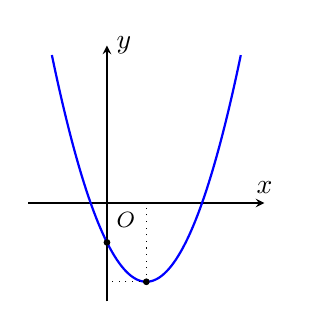
\begin{tikzpicture}[>=stealth,scale=0.5] 
			\draw[->,black] (-2,0) -- (4,0)node[above] {$x$};
			\draw[->,black] (0,-2.5) -- (0,4)node[right] {$y$}; 
			\node at (0,0) [below right] {\footnotesize $O$}; 
			\draw[smooth,blue,thick,samples=100,domain=-1.4:3.4] plot(\x,{(\x)^2-2*(\x)-1}); 
			\draw[dotted] 
			(1,-2) -- (1,0) (1,-2) -- (0,-2);
			\fill[fill=black,draw=black] 
			(1,-2) circle (2pt)
			(0,-1) circle (2pt);
			\end{tikzpicture}}
		
		\loigiai
		{
			Dựa vào dạng đồ thị suy ra $ a > 0; $\\
			Giao điểm với trục $ Oy $ có tung độ âm $ \Rightarrow c < 0; $\\
			Đỉnh của $ (P) $ có hoành độ dương nên $ -\dfrac{b}{2a} > 0  $ hay $ b < 0.$\\
			Vậy $ a > 0, b < 0, c < 0. $
		}
	\end{ex}
	
	\begin{ex}%[0D2B3]
		Cho parabol $y=ax^2+bx+4$ có trục đối xứng là đường thẳng $x=\dfrac{1}{3}$ và đi qua điểm $A(1;3)$. Tổng giá trị $a+2b$ là
		\choice
		{\True $1$}
		{$-1$}
		{$-\dfrac{1}{2}$}
		{$\dfrac{1}{2}$}
		\loigiai{
			\begin{itemize}
				\item [$\bullet$] Trục đối xứng $x=-\dfrac{b}{2a}=\dfrac{1}{3} \Leftrightarrow 2a+3b=0 \quad (1)$.
				\item [$\bullet$] Đồ thị qua điểm $A(1;3)$ nên $a+b+4=3 \Leftrightarrow a+b =-1 \quad (2)$.
			\end{itemize}
		Từ (1) và (2) ta được hệ $\heva{&2a+3b=0\\&a+b=-1 } \Leftrightarrow \heva{&a=-3\\&b=2}$. Suy ra $a+2b =1$.
		}
	\end{ex}
\begin{ex}%[Bùi Thanh Cương, Tex45-THPT-04]%[0D2K3-3]%
	\immini
	{
		Cho hàm số $y=ax^2+bx+c$ có đồ thị như hình bên. Tính tổng $a+b+c$.
		\haicot
		{\True $0$}
		{$-1$}
		{$1$}
		{$2$}
	}
	{
		\begin{tikzpicture}[x=0.8cm,y=0.8cm,>=stealth]
			\draw[->] (-3,0) -- (2.5,0) node[above]{\scriptsize $x$};
			\draw[->] (0,-3.5) -- (0,1.5) node[left]{\scriptsize $y$};
			\draw (0.1,0.1) node[below left]{\scriptsize $O$};
			\foreach \i in {-1}{
				\draw (\i,0) node[above]{\scriptsize $\i$};
				\draw (0,\i) node[left]{\scriptsize $\i$};
				\draw (0.12,\i) -- (-0.12,\i) (\i,0.12) -- (\i,-0.12);}
			\draw[samples=100,domain=-1.7:1.2,blue] plot (\x,{2*(\x)^2+(\x)-3});
			\draw (0.9,0.08) node[above]{\scriptsize $1$}; 
		\end{tikzpicture}
	}
	\loigiai
	{
		Đồ thị hàm số đi qua điểm $(1;0)$. Do đó $0=a+b+c$.
	}
\end{ex}

\begin{ex}%[Trần Mạnh Hùng]%[0D4B5]
	Cho tam thức $f(x)=ax^2+bx+c$, với $a\ne 0$ và $\Delta=b^2-4ac=0$. Khẳng định nào sau đây \textbf{sai}?
	\choice
	{\True $f(x)$ luôn cùng dấu với hệ số $a$}
	{$a.f(x)=0$ khi và chỉ khi $x=-\dfrac{b}{2a}$}
	{$a.f(x)>0 ,\;\forall x\in\mathbb{R}\backslash\left\{-\dfrac{b}{2a}\right\}$}
	{Đồ thị hàm số $y=f(x)$ cắt $Ox$ tại một điểm duy nhất}
\end{ex}

\begin{ex}%[Trần Mạnh Hùng]%[0D4B5]
	Bảng xét dấu sau đây là của một trong số bốn tam thức bậc hai được cho dưới đây. Hỏi đó là tam thức nào?
	\begin{center}
		
\begin{tikzpicture} 
			\tkzTabInit[lgt=2]
			{$x$/1,$f(x)$/1}
			{$-\infty$,$1$,$2$,$+\infty$}
			\tkzTabLine{ , +, 0, -, 0,+,}
		\end{tikzpicture}
	\end{center}
	\choice
	{$f(x)=x^2-2x+3$}
	{$f(x)=x^2-2x-3$}
	{\True $f(x)=x^2-3x+2$}
	{$f(x)=-x^2+3x-2$}
\end{ex}

\begin{ex}%[TRẦN VĂN THIỆN NGỌC]%[0D4B5]
	Tập nghiệm của bất phương trình $-3x^2+2x+1<0$ là
	\choice
	{\True $\left(-\infty;-\dfrac{1}{3}\right)\cup \left(1;+\infty\right)$}
	{$\mathbb{R} \setminus \left\{-\dfrac{1}{3};1\right\}$}
	{$\left(-\dfrac{1}{3};1\right)$}
	{$\mathbb{R}$}
\end{ex}

\begin{ex}%[0D4K5-2]
	Tam thức $f(x)=3x^2+2(2m-1)x+m+4$ dương với mọi $x \in \mathbb{R}$ khi và chỉ khi
	\choice
	{\True $-1<m<\dfrac{11}{4}$}
	{$-\dfrac{11}{4}<m<1$}
	{$-\dfrac{11}{4}\le m\le 1$}
	{$m<-1$ hoặc $m>\dfrac{11}{4}$}
	\loigiai
	{
		Tam thức $f(x)$ có $a=3>0$. Do đó
		\begin{eqnarray*}
			f(x)>0,\forall x \Leftrightarrow \Delta'<0 \Leftrightarrow (2m-1)^2-3(m+4)<0 \Leftrightarrow 4m^2-7m-11<0 \Leftrightarrow -1<m<\dfrac{11}{4}.
		\end{eqnarray*}
		Vậy $-1<m<\dfrac{11}{4}$ là các giá trị thỏa mãn yêu cầu bài toán.
	}
\end{ex}

\begin{ex}
	Số nghiệm của phương trình $\sqrt{x^{2}+4x-2}=x-3$ là
	\choice
	{\True 0}
	{1}
	{2}
	{3}
	\loigiai{
	Bình phương hai vế ta được
	$$x^2+4x-2=x^2-6x+9 \Leftrightarrow x=\dfrac{11}{10}$$
	Thử lại, ta thấy không thoả nên phương trình vô nghiệm.
}
\end{ex}
\begin{ex}%[0D2G3-5]%[]%
	Một doanh nghiệp tư nhân $A$ chuyên kinh doanh xe gắn máy các loại. Hiện nay doanh nghiệp đang tập trung chiến lược vào kinh doanh xe honda Future Fi với chi phí mua vào một chiếc là $27$ (triệu đồng) và bán với giá $31$ (triệu đồng) mỗi chiếc. Với giá bán này thì số lượng xe mà khách hàng sẽ mua trong một năm là $600$ chiếc. Nhằm mục tiêu đẩy mạnh hơn nữa lượng tiêu thụ dòng xe đang ăn khách này doanh nghiệp dự định giảm giá bán và ước tính rằng nếu giảm $1$ (triệu đồng) mỗi chiếc thì số lượng xe bán ra trong một năm sẽ tăng thêm $200$ chiếc. Vậy doanh nghiệp phải định giá bán mới là bao nhiêu để sau khi đã thực hiện giảm giá lợi nhuận thu được sẽ là cao nhất?
	\choice
	{\True $30,5$ triệu}
	{$29,5$ triệu}
	{$30$ triệu}
	{$29$ triệu}
	\loigiai
	{
		Gọi $x$ ( đơn vị: triệu đồng) là giá bán mới. Khi đó số tiền đã giảm là: $31-x$ \, ($0<x<31$). \\
		Số lượng xe tăng lên là: $200(31-x)$.\\
		Vậy tổng số sản phẩm bán được là: $600+ 200(31-x ) =6800-200x$.\\
		Doanh thu mà doanh nghiệp sẽ đạt được là: $(6800 -200x)x$.\\
		Tiền vốn mà doanh nghiệp phải bỏ ra là: $(6800 -200x)27$.\\
		Lợi nhuận mà công ty đạt được sẽ là:
		\[L(x)= \text{Doanh thu} -\text{Tiền vốn} =(6800 -200x)x-(6800 -200x)27=-200x^2+12200x-183600.\]
		Ta có biểu thức $L(x)$ là một parabol có đỉnh $I(30,5;2450)$ và có bảng biến thiên như sau:
		\begin{center}
			\begin{tikzpicture}
				\tkzTabInit[lgt=1.5,espcl=2.0,deltacl=.5,nocadre]
				{$x$ /0.7,$L(x)$ /1.7}
				{$0$ , $30{,} 5$ , $31$}
				%\tkzTabLine{,-,0,+,0,-,}
				\tkzTabVar{-/$-183600$ ,+/$2450$, -/$2400$}
			\end{tikzpicture}
		\end{center}
		Từ bảng biến thiên suy ra $L(x)_{\max} =2450$ khi $x=30,5$ triệu. Vậy giá bán mới $30,5$ triệu đồng.
	}
\end{ex}
\centerline{---HẾT---}
\Closesolutionfile{ans}
